\chapter{Sistema de vinculación de componentes}\label{ch:sistema-de-vinculacion-de-componentes}

En este capítulo se abordará la creación de un sistema de
vinculación de componentes para \textit{JAMS}, empezando por
la estructura de un componente y terminando por la carga
del mismo dentro de \textit{JAMS}.

\section{Estructura de un componente}\label{sec:estructura-de-un-componente}

Los componentes, al igual que en muchas aplicaciones \textit{Java},
están conformados por un archivo \textit{jar} con el código que
se desea usar en la aplicación principal.
Más concretamente, un componente de \textit{JAMS} debe contener
dos elementos esenciales:
\begin{itemize}
    \item \textbf{Punto de entrada}: está conformado por una
    clase que extiende a $Plugin$.
    \textit{JAMS} crea una instancia de esta clase para
    poder ejecutar el código externo.
    \item \textbf{Archivo de metadatos}: confirmado por un archivo
    $plugin.json$ en la raíz del archivo \textit{jar}.
    Este archivo contiene los parámetros globales del componente,
    como pueden ser el \textbf{nombre}, la dirección del
    \textbf{punto de entrada}, la versión, los autores,
    o la descripción.
    Un ejemplo de archivo $plugin.json$ se puede observar en la
    figura \ref{fig:plugin-json}.
\end{itemize}


\begin{figure}[h]
    \centering
    \begin{lstlisting}[frame=single,label={lst:plugin-json}]
{
  "name": "NES4JAMS",
  "main": "io.github.gaeqs.nes4jams.NES4JAMS",
  "version": "0.1-ALPHA",
  "authors": [
    "Gael Rial Costas"
  ],
  "favicon": "/gui/icon/favicon.png",
  "description_node": "NES4JAMS_DESCRIPTION"
}
    \end{lstlisting}
    \caption{Ejemplo de archivo $plugin.json$}
    \label{fig:plugin-json}
\end{figure}

\subsection{Dependencias}\label{subsec:dependencias}

Un componente puede depender de otro componente.
Para proporcionar una inicialización de los componentes
correcta se proporcionan los parámetros $dependencies$
y $soft\_dependencies$, los cuales se pueden utilizar en
el archivo $plugin.json$.
Todos los componentes cuyo nombre esté dentro de una de estas
listas será inicializado antes.
Si no se encuentra ningún componente que tenga el nombre
de algún valor de $dependencies$, el componente no
se inicializará, lanzando una excepción.
Cabe destacar que dos componentes no pueden conformar
una \textbf{dependencia cíclica}.

\subsection{Puntos de entrada}\label{subsec:puntos-de-entrada}

Como ya se ha mencionado, un punto de entrada está conformado
por una \textbf{clase que extiende a $Plugin$}.
El desarrollador puede extender dos métodos definidos por esta clase:
$onEnable$ y $onEnable$, los cuales serán llamados cuando el
componente es vinculado o desvinculado de la aplicación principal.
Un ejemplo de punto de entrada se puede observar en la figura \ref{fig:entry-point}.

\begin{figure}[h]
    \centering
    \begin{lstlisting}[frame=single,label={lst:entry-point},language=Kotlin]
class MyPlugin : Plugin() {

    override fun onEnable() {
        println("My plugin has been enabled!")
        if (JamsApplication.isLoaded()) {
            loadApplicationData()
        }
    }

    override fun onDisable() {
        println("My plugin has been disabled!")
    }

    @Listener
    fun onApplicationLoad(event: JAMSApplicationPostInitEvent)
        = loadApplicationData()

    private fun loadApplicationData() {
        println("Now I can access the JavaFX application!")
    }

}
    \end{lstlisting}
    \caption{Ejemplo de punto de entrada de un componente desarrollado en \textit{Kotlin}}
    \label{fig:entry-point}
\end{figure}

 El punto de entrada puede ser inicializado en diferentes
etapas del proyecto: el componente será cargado antes del contexto
de \textit{JavaFX} si este ya estaba instalado en la aplicación
cuando esta es lanzada.
Es por eso que el desarrollador debe \textbf{comprobar si el contexto ha sido creado}
antes de añadir o modificar nuevos elementos.
Si el contexto aún no ha sido creado, los componentes podrán
usar el evento $JAMSApplicationPostInitEvent$ para ejecutar
código cuando este sea inicializado.
Este sistema de eventos se verá en profundidad en esta memoria más adelante.


\section{Vinculación de un componente}\label{sec:vinculacion-de-un-componente}

Un componente puede ser vinculado de dos maneras diferentes:
cuando el usuario \textbf{instala el componente} desde la aplicación
y cuando la \textbf{aplicación principal es inicializada} y el componente
está ya instalado.
La vinculación de componentes difiere en varios aspectos en estas
dos situaciones: cuando el componente es instalado, \textit{JAMS}
comprueba si \textbf{todas sus dependencias fuertes están presentes}.
Si esto no se cumple, el componente no puede ser instalado.
Cuando la aplicación principal es inicializada esta debe vincular
una cantidad no definida de componentes.
Es por ello que debe generar un \textbf{grafo de dependencias}
antes de inicializar los componentes.

\section{Desvinculación de un componente}\label{sec:desvinculacion-de-un-componente}

Un componente es desvinculado de la aplicación principal
cuando el usuario \textbf{desinstala el componente} desde
la aplicación o cuando la \textbf{aplicación principal es cerrada}.
De la misma manera que en la vinculación, el proceso de
desvinculación \textbf{difiere} en ambas circunstancias.
Para que un componente sea desinstalado, el usuario
debe desinstalar previamente \textbf{todos los componentes
que dependen} del componente a desinstalar.
Solo cuando no exista ningún componente dependiente
es cuando se puede desinstalar el componente deseado.
Cuando la aplicación principal es cerrada
\textbf{no se desvincula ningún componente},
únicamente se llama al método $onDisable$, dejando
el proceso de desvinculación a la \textit{JVM}.

\section{Interfaz de usuario}\label{sec:interfaz-de-usuario}

Los usuarios pueden instalar o desinstalar componentes
desde la \textbf{ventana de configuración}.
En esta interfaz se mostrará la lista de componentes
que están instalados junto con el nombre, la versión
y la descripción de estos.

\begin{figure}[h]
    \centering
    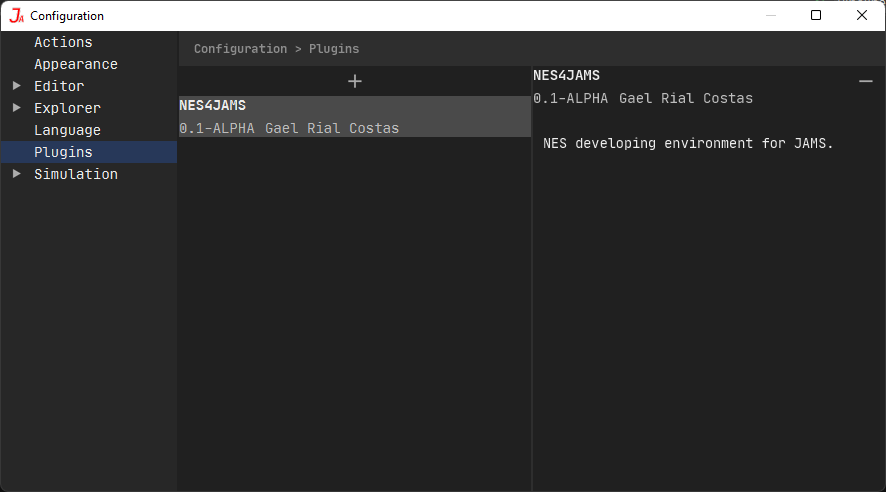
\includegraphics[width=\textwidth]{images/componentes/plugin-ui}
    \caption{Sección de componentes en la configuración}
    \label{fig:plugin-ui}
\end{figure}